\section{Motors}
This section will propose two different possible types of motors Hades could end up using.

\subsection{AC motor}
AC motors consist of two main part. A stator and a rotor. The stator is a stationary part and the rotor is a rotating part. The rotor is located inside of the stator and due to magnetic fields inside of the stator, the rotor will rotate.\\ 
AC motor use a alternative current see figure\ref{fig:ACmotor}. Due to the slip-rings, the AC motor transfers energy to the robot.

\begin{figure}[h]
    \centering
    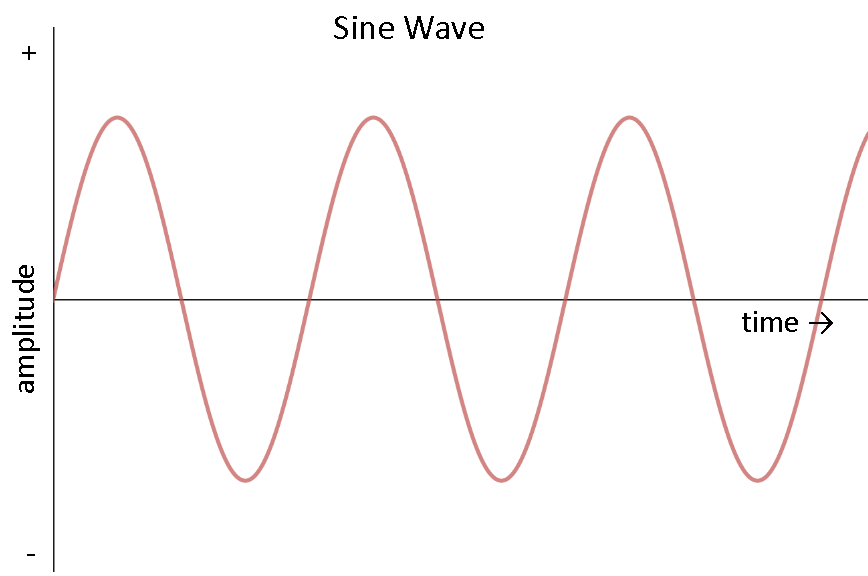
\includegraphics[width=.6\linewidth]{figures/wave.png}
    \caption{Alternative current\cite{ACmotor3}}
    \label{fig:ACmotor}
\end{figure}

\subsection{Brushless DC motor}
The working process of a brushless DC motor is similar to an AC motor. The main difference between a brushless DC motor and an AC motor is how they produce energy. Furthermore, brushless DC motors are connected to the robot with a commutator instead of slip rings. The brushless DC motor transfers direct current energy to the robot. The brushless DC working output is not steady but always in the same direction\ref{fig:DCmotor}.

\begin{figure}[h]
    \centering    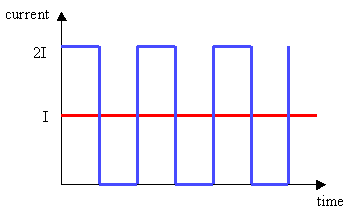
\includegraphics[width=.6\linewidth]{figures/dcMotor.png}
    \caption{Brushless DC curve angular\cite{DCbrusshles}}
    \label{fig:DCmotor}
\end{figure}

 %\newpage

%conclusion  - put them up against each other